% !TEX TS-program = xelatex
% !TEX encoding = UTF-8 Unicode

\documentclass[a4paper,10pt]{article}
\usepackage{latexsym}
\usepackage[empty]{fullpage}
\usepackage{titlesec}
\usepackage{marvosym}
\usepackage[T1]{fontenc}
\usepackage{fontspec}
\usepackage{tikz}
\usetikzlibrary{shapes,calc}
\usepackage{xcolor}
\usepackage{lipsum}
\usepackage{ragged2e}
\usepackage{etoolbox}
\usepackage{ifmtarg}
\usepackage{ifthen}
\usepackage{pgffor}
\usepackage{marvosym}
\usepackage{parskip}
\usepackage[absolute,overlay]{textpos}
\usepackage[left=7.6cm,top=1cm,right=1cm,bottom=0.8cm,nohead,nofoot]{geometry}
\usepackage[hidelinks]{hyperref}
\usepackage{fontawesome5}
\usepackage{setspace}
\usepackage{ifthen}
\usepackage{datetime}
\usepackage{enumitem}
\usepackage{graphics}
\usepackage{pdfpages}
\hypersetup{
	pdftitle={Morteza Karimi CV},
	pdfauthor={Morteza Karimi},
	pdfsubject={Morteza Karimi Web Develpoer CV},
	pdfkeywords={CV,Resume,Morteza Karimi,Web Developer,Back-end Developer,Front-end Developer},
	colorlinks=false,
	allbordercolors=white
}
\graphicspath{{images/}}
%\import{./logo2.eps_tex}{logo2.eps_tex}
%%%%%%%%%%%%%%%%%%%%%%%%%% definitions %%%%%%%%%%%%%%%%%%%%%%%%%%%%%%%%%%%%%%5
\definecolor{defaultfontcolor}{HTML}{212121}
\definecolor{white}{RGB}{224,224,224}
\definecolor{gray}{HTML}{4D4D4D}
\definecolor{bootstrapSecondary}{HTML}{6c757d}
\definecolor{sidecolor}{HTML}{212121}
\definecolor{sidetextcolor}{RGB}{224,224,224}
\definecolor{mainblue}{HTML}{5AB9EA}
\definecolor{maingreen}{HTML}{52D3AA}
\definecolor{maingray}{HTML}{B9B9B9}

\newdateformat{usvardate}{%
	\monthname[\THEMONTH] \ordinal{DAY}, \THEYEAR}

\pagestyle{empty} % Disable headers and footers

%%%%%%%%%%%%%%%%%%%%%%%%%% Margin %%%%%%%%%%%%%%%%%%%%%%%%%%%%%%%%
\setlength{\parindent}{5pt} % Disable paragraph indentation
\renewcommand{\baselinestretch}{1.3} 
\setlength{\TPHorizModule}{1cm} % Left margin
\setlength{\TPVertModule}{6cm} % Top margin

%%%%%%%%%%%%%%%%%%%%%% Profile Picture %%%%%%%%%%%%%%%%%%%%%%%%%%%%%%
\newlength\imagewidth
\newlength\imagescale
\pgfmathsetlength{\imagewidth}{3cm}
\pgfmathsetlength{\imagescale}{\imagewidth/600}
\newcommand{\profilepic}[1]{\renewcommand{\profilepic}{#1}}

%%%%%%%%%%%%%%%%%%%%%%% birthday %%%%%%%%%%%%%%%%%%%%%%%%
\newdate{birthday}{17}{06}{1994}
\newcommand{\birthdate}{\usvardate\displaydate{birthday}}

\makeatletter
%%%%%%%%%%%%%%%%%%% change default color %%%%%%%%%%%%%%%%%%%%
\newcommand{\globalcolor}[1]{%
	\color{#1}\global\let\default@color\current@color
}

%%%%%%%%%%%%%%%%%%%%%%%%%% New Commands %%%%%%%%%%%%%%%%%%%%%%%%%%
\newcommand{\resumeItem}[6][]{
	\ifthenelse{\equal{#1}{}}{\subsection*{#2}}{\subsection*{\href{#1}{#2}}}
	{\normalsize #3}\\
	\textcolor{bootstrapSecondary}{
%		\ifthenelse{\equal{#4}{}}{}{\small{#4}{ / }}
		{\small#5}
	}\\\\
	{#6}
}

\newcommand{\resumeSubheading}[3]{\textbf{#1} & \small\textcolor{bootstrapSecondary}{#2} \\
		{\small#3}\\\\
%		\ifthenelse{\equal{#1}{}}{}{\tiny{\textbf{Thesis Title:} #1 }&\\}
}
\newcommand{\resumeSubHeadingListStart}{\begin{tabular*}{\textwidth}{@{}l@{\extracolsep{\fill}}l}}
\newcommand{\resumeSubHeadingListEnd}{\end{tabular*}}%\vspace{-5pt}}
\renewcommand{\labelitemi}{$\bullet$}
\renewcommand{\labelitemii}{$\circ$}
%%%%%%%%%%%%%%%%%%%% Side Section Rule %%%%%%%%%%%%%%%%%%%%%%%%%%%%%%%%%%55
\newcommand{\siderule}{
	\vspace*{0.5\baselineskip}
	\hrule\@height 2pt
	\vspace*{0.5\baselineskip}
}
%%%%%%%%%%%%%%%%%%%%%%%%%%% Content Item %%%%%%%%%%%%%%%%%%%%%%%%%%%%%%%%%%%%%%
\newcommand{\contactItem}[3][]{%
	\textcolor{maingreen}{\Large{#2}} &
	 {
		\ifthenelse{\equal{#1}{}}
		{
			#3
		}{
		\href{#1}{#3}
		}
	}
\\
}

%%%%%%%%%%%%%%%%%%%%%%%%%%%%%% Skills Item %%%%%%%%%%%%%%%%%%%%%%%%%%%%%%%%
\newcounter{circle}
\newcommand{\skillItem}[2]{%
	\textbf{#1}\hfill
	\textcolor{maingreen}{
		\setcounter{circle}{0}
		\whiledo {\value{circle} < #2}%
		{%
			\small\faCircle\,
			\stepcounter {circle}%
		}
		\whiledo {\value{circle} < 5}%
		{%
			\small\faCircle[regular]\,
			\stepcounter {circle}%
		}
	}\\
}
%%%%%%%%%%%%%%%% Profile Section in side panel %%%%%%%%%%%%%%%%%%%%%%%%%%%%%%%%%%%%%%%%
\newcommand{\makeprofile}{
	%%%%%%%%%%%%% side background %%%%%%%%%%%%%%%%%%%%%
	\begin{tikzpicture}[remember picture,overlay]
	\node [rectangle, fill=sidecolor, anchor=north, minimum width=9cm, minimum height=\paperheight+1cm] (box) at (-6cm,1.5cm){};
	\end{tikzpicture}
	%%%%%%%%%%%%%%% text block %%%%%%%%%%%%%%%%%%%%%
	\begin{textblock}{5}(0.5, 0.2)
		\textcolor{sidetextcolor}{
			%%%%%%%%%%%%%%%%%%%% profile pic %%%%%%%%%%%%%%%%%%%%%%%%%%
			\ifthenelse{\equal{\profilepic}{}}{}{
				\begin{center}
					\begin{tikzpicture}[x=\imagescale,y=-\imagescale]
					\clip (600/2, 600/2) circle (600/2);
					\node[anchor=north west, inner sep=0pt, outer sep=0pt] at (1,0) {\includegraphics[width=\imagewidth]{\profilepic}};
					\end{tikzpicture}
				\end{center}
			}
			%%%%%%%%%%%%%%%%%%%% Contact Section %%%%%%%%%%%%%%%
			\section*{Contact}\siderule
				\begin{spacing}{1.5}
					\begin{tabular}{c l}
%					\contactItem{\faBirthdayCake}{\birthdate}
%					\contactItem{\faRing}{Married}
					\contactItem[tel:+989216351266]{\faMobile*}{+98 921 635 1266}
					\contactItem{\faMapMarker*}{Tehran, Iran}
					\contactItem[https://morteza-karimi.ir]{\faGlobe}{morteza-karimi.ir}
					\contactItem[mailto:me@morteza-karimi.ir]{\faEnvelope}{me@morteza-karimi.ir}
					\contactItem[https://www.linkedin.com/in/MortezaKarimi]{\faLinkedin}{MortezaKarimi}
					\contactItem[https://github.com/MortezaKarimi]{\faGithub}{MortezaKarimi}
					\contactItem[https://stackoverflow.com/story/MortezaKarimi]{\faStackOverflow}{MortezaKarimi}
					\end{tabular}
				\end{spacing}
			\vspace*{-0.3\baselineskip}
			%%%%%%%%%%%%%%%%%%%% Hard Skills Section %%%%%%%%%%%%%%%
			\section*{Hard Skills}\siderule
				\vspace*{0.4\baselineskip}
				\begin{spacing}{1.5}
					\skillItem{PHP}{4}
					\skillItem{Python}{3}
					\skillItem{JavaScript}{3}
					\skillItem{Yii2}{4}
					\skillItem{Laravel}{3}
					\skillItem{React.JS}{2}
					\skillItem{Vue.JS}{2}
					\skillItem{Node.JS}{2}
					\skillItem{Tensorflow}{2}
					\skillItem{OpenCV}{2}
				\end{spacing}
			\vspace*{-\baselineskip}
			\section*{Interests}\siderule
			\vspace*{0.4\baselineskip}
			\begin{spacing}{1.5}
				\resizebox{\linewidth}{!}{%
				\begin{tabular}{cccc}
				\huge\faLaptopCode&
				\huge\faRunning&
				\huge\faSuitcaseRolling&
				\huge\faMugHot\\
				\end{tabular}
			}
			\end{spacing}
		\vspace*{-0.3\baselineskip}
		%%%%%%%%%%%%%%%%%%%% Languages Section %%%%%%%%%%%%%%%
		\section*{Languages}\siderule
		\vspace*{0.4\baselineskip}
		\begin{spacing}{1.5}
			\skillItem{Persian}{4}
			\skillItem{English}{2}
		\end{spacing}		
		}
	\end{textblock}
}

\makeatother

\profilepic{morteza.jpg}
\author{Morteza Karimi}
\title{Web Developer}

\makeatletter
%%%%% Set default color %%%%%
\AtBeginDocument{\globalcolor{defaultfontcolor}}
\begin{document}
%	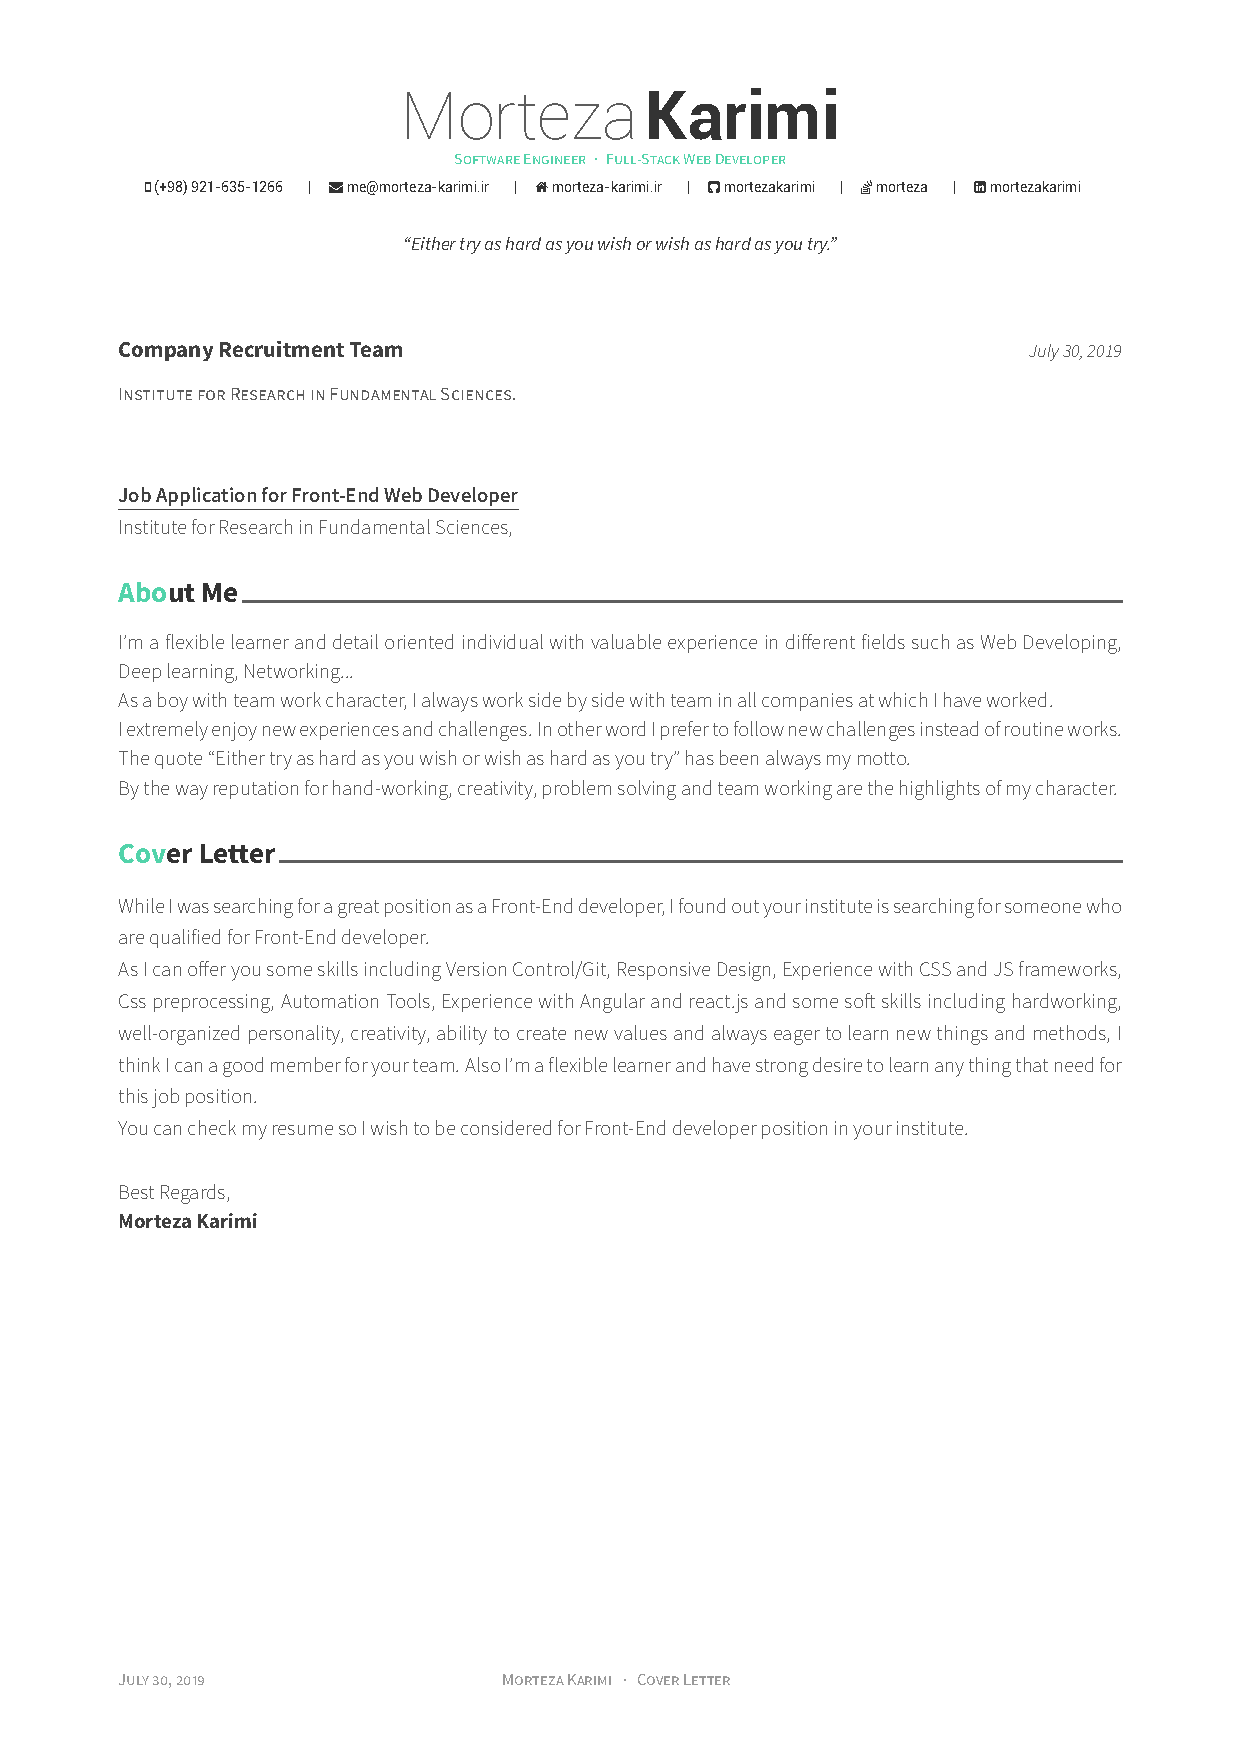
\includepdf{./CoverLetter/morteza-karimi-coverletter.pdf}
	\newpage
	\makeprofile
	\noindent
	{\Huge\janeroe \textbf{\@author}}\\[0.2\baselineskip]
	{\large\janeroe\@title}
	\section*{About Me}\hrule
	I'm a flexible learner and detail oriented individual with valuable experience in different fields such as Web Developing, Deep learning, Networking...\\
	As a boy with team work character, I always work side by side with team in all companies at which I have worked.\\
	I extremely enjoy new experiences and challenges. In other word I prefer to follow new challenges instead of routine works. The quote ``Either try as hard as you wish or wish as hard as you try" has been always my motto.\\
	By the way reputation for hand-working, creativity, problem solving and team working are the highlights of my character.
	\section*{Education}\hrule
	\resumeSubHeadingListStart
	\resumeSubheading{Shahrood University of Technology}{2017 - Present}{Master of Science in Artificial Intelligence; GPA: 3.77 (16.46/20)}
	\resumeSubheading{Khayyam University of Mashhad}{2012 - 2017}{Bachelor of Engineering in Software Engineering; GPA: 3.17 (15.47/20)}
	\resumeSubHeadingListEnd
	
	\vspace*{-1\baselineskip}
	\section*{Experience}\hrule
	\resumeItem[http://heyzha.ir/]{Heyzha Programming Co}{Web Application Developer}{Iran, Sabzevar}{2017 - 2019}{
	Cooperation with Heyzha company was a great spark for success in my work life. I did lots of project in this company. At first I started my work with solving the problems of a website with Laravel framework. Also I developed other websites with Yii2 framework and it followed a great impact because it caused 33\%  improvement in all the projects of Heyzha company. In the same way the income of company for developing more and more projects had improved, So the company experienced an up ward trend. By the way I experienced such a great challenges in designing complicated portals.
	}
	\resumeItem[http://khayyam.ac.ir/]{Khayyam University of Mashhad}{Back-End Web developer}{Iran, Mashhad}{2014 - 2016}{
	In Khayyam university I had a game project. Its name was tik-tak-toe that was in relation with IOS app. For developing it, I used node.js platform and socket.io library. Also I experience a team work project in this university. It was developing Khayyam university culture center website. Actually because of my good background in bachelor final project, use node.js and PHP together, this great project was given to me.
	}
	\newpage
	\makeprofile
	\noindent
	\resumeItem{Freelance Experience}{Full-Stack Web developer}{Iran, Mashhad}{2012 - Present}{
	\vspace*{-2\baselineskip}
	\begin{itemize}[leftmargin=*]
		\item Promac Co.\\
		For the first time I used my admin panel in developing this website, so it followed a great impact and it was the satisfaction of employer.
		\item Rastegary charity website\\
		It's one of my freelance works in the early years of my work field of web developing.\\ I tried to use PHP MVC framework Yii And UI framework Bootstrap in this web project.\\
		The first ideas of building my custom admin module for the next projects was occurred during developing this project that was very useful for my future projects.
		\item Variable project\\
		I've done different kind of student projects that included website design and android application.\\I worked with electron framework, Qt C++ framework, python language and many other techniques in these projects.\\
	\end{itemize}
	}
	\section*{Volunteer Experience}\hrule
	\resumeItem{Artificial Intelligence projects}{Programmer}{}{2017 - Present}{
	Because of my intrest in Image Processing field, voluntary I worked on image processing projects.\\Also based on my information about deep learning I started working on a project, that is about forecasting financial markets which is currently underway.}
	\resumeItem[https://morteza-karimi.ir/gentelella-rtl/public/]{Create RTL template based on Gentelella theme}{Front-End \& Translate}{}{2014 - Present}{
	Sharing my abilities and information in translating and RTL on open source template was one of my great work experience.\\By searching in google I found out a useful template so I worked on it because having good and free template could be useful for web developers.\\ I got familiar with different tools in this project and got many feedback from many people all around the world that helped me in developing this project.  
	}
	\newpage
	\makeprofile
	\noindent
	
	\resumeItem[https://valencia.ir/]{Valencia fan club website in Iran}{Full-Stack Web developer}{}{2014}{
	I started my first work experience in field of ``web developing" with designing 0 to 100 Valencia fan club website. I had a serious plan for developing this website that led to my employer satisfaction. I used Yii framework for this website to create complicated system such as like, comment and ... efficiently.
	}
	\resumeItem{Web Development Teacher}{Teacher}{}{2014 - 2019}{I always like to share my information with others so I like to have some experiences in designing open source projects or teaching my information to others. So I decided to  schedule and plan some courses to teach web development lessons to my students.}
\end{document}
